%%%%%%%%%%%%%%%%%%%%%%%%%%%%%%%%%%%%%%%%%%%%%%%%%%%%%%%%%%%%%%%%%%%%%%%%
%                                                                      %
%     File: Thesis_Appendix_A.tex                                      %
%     Tex Master: Thesis.tex                                           %
%                                                                      %
%     Author: Andre C. Marta                                           %
%     Last modified :  2 Jul 2015                                      %
%                                                                      %
%%%%%%%%%%%%%%%%%%%%%%%%%%%%%%%%%%%%%%%%%%%%%%%%%%%%%%%%%%%%%%%%%%%%%%%%

\chapter{Extra plots}
\label{chapter:extra_plots}

\begin{figure}[h]
	\centering
		\centering
		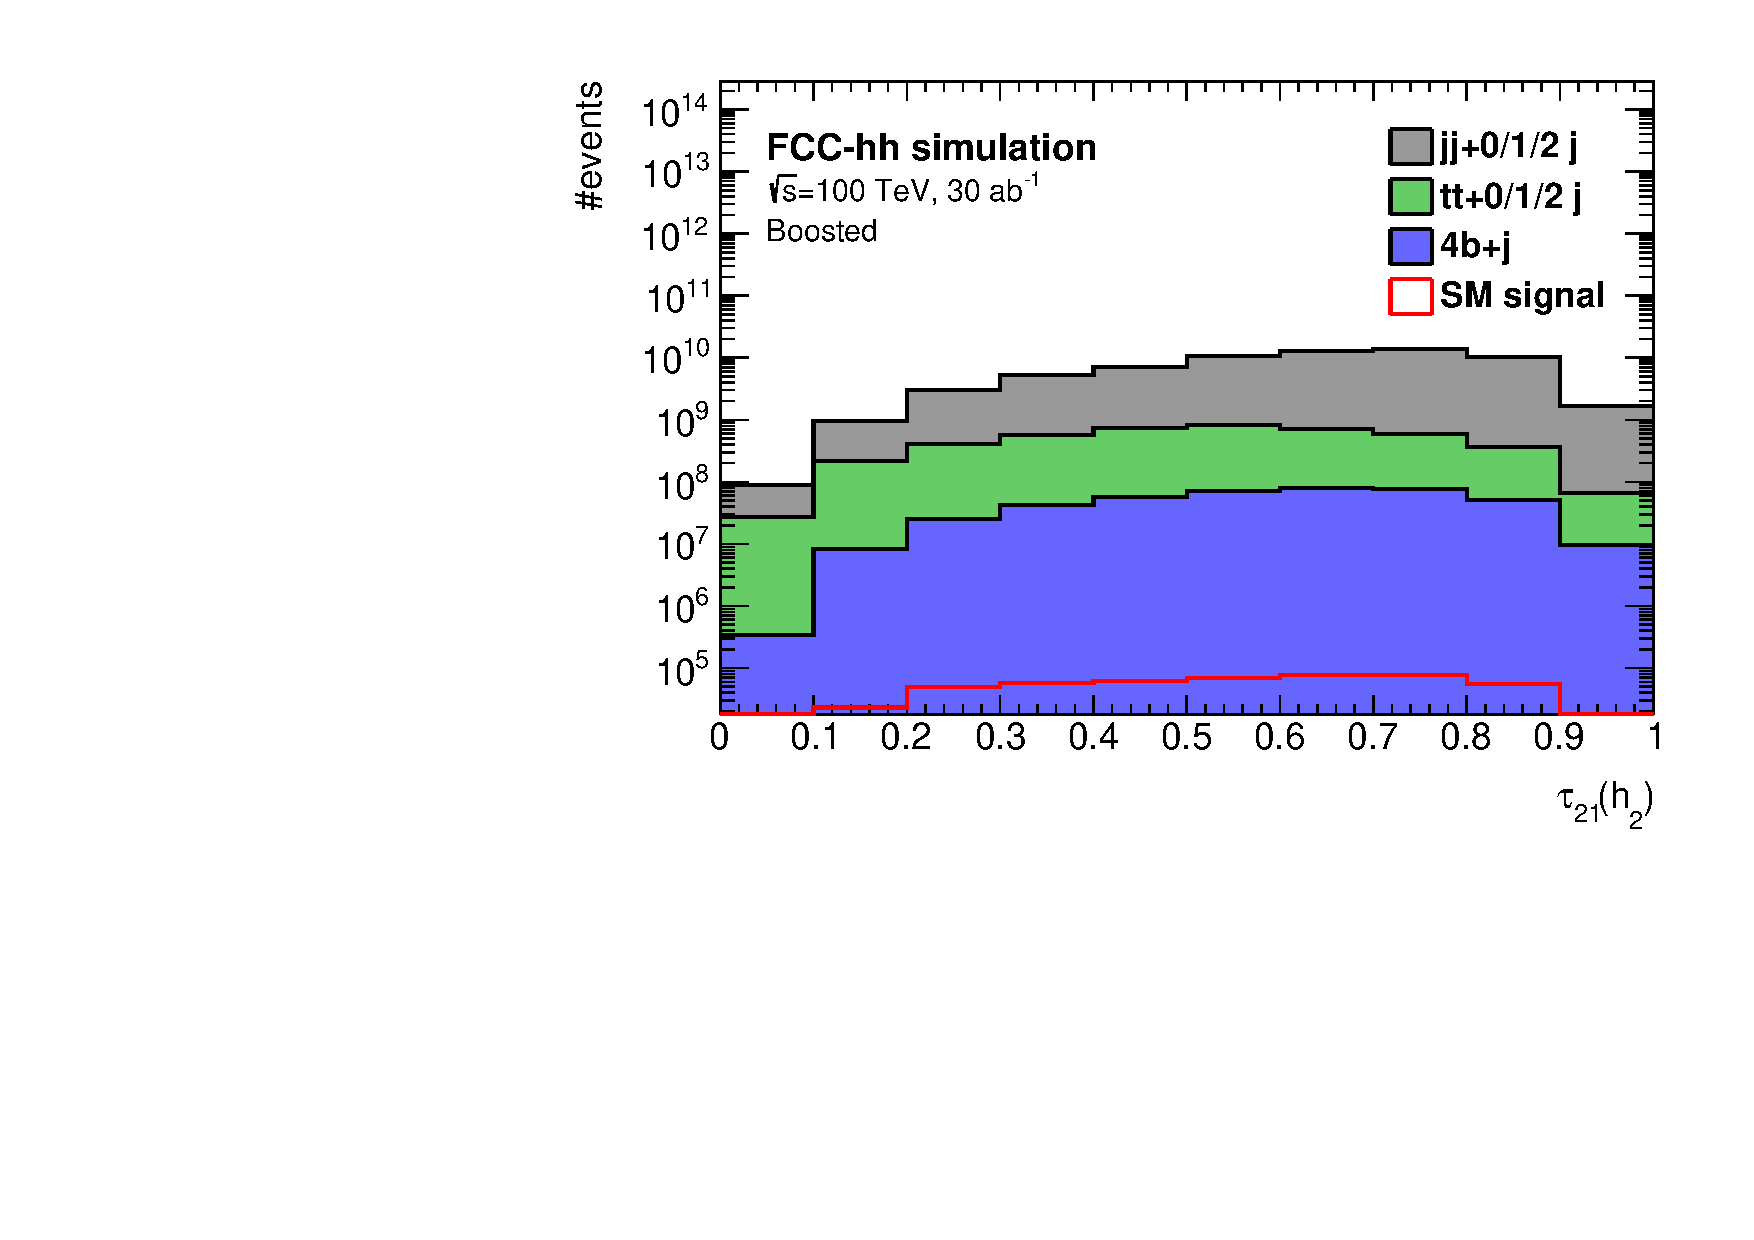
\includegraphics[trim={.65cm 0 0 0},clip,width=0.5\linewidth]{./Figures/hist_h2_tau21_stack.pdf}
		%\caption{oi}
		%\label{fig:h1_pt}
	\caption{$\tau_{21}$ distribution for the sub leading Higgs candidate for the baseline analysis. The histogram is normalized to $\mathcal{L}=30~\text{ab}^{-1}$.}
	\label{fig:tau21_h2_stack}
\end{figure} 

\begin{figure}[h]
	\centering
	\begin{minipage}{.5\textwidth}
		\centering
		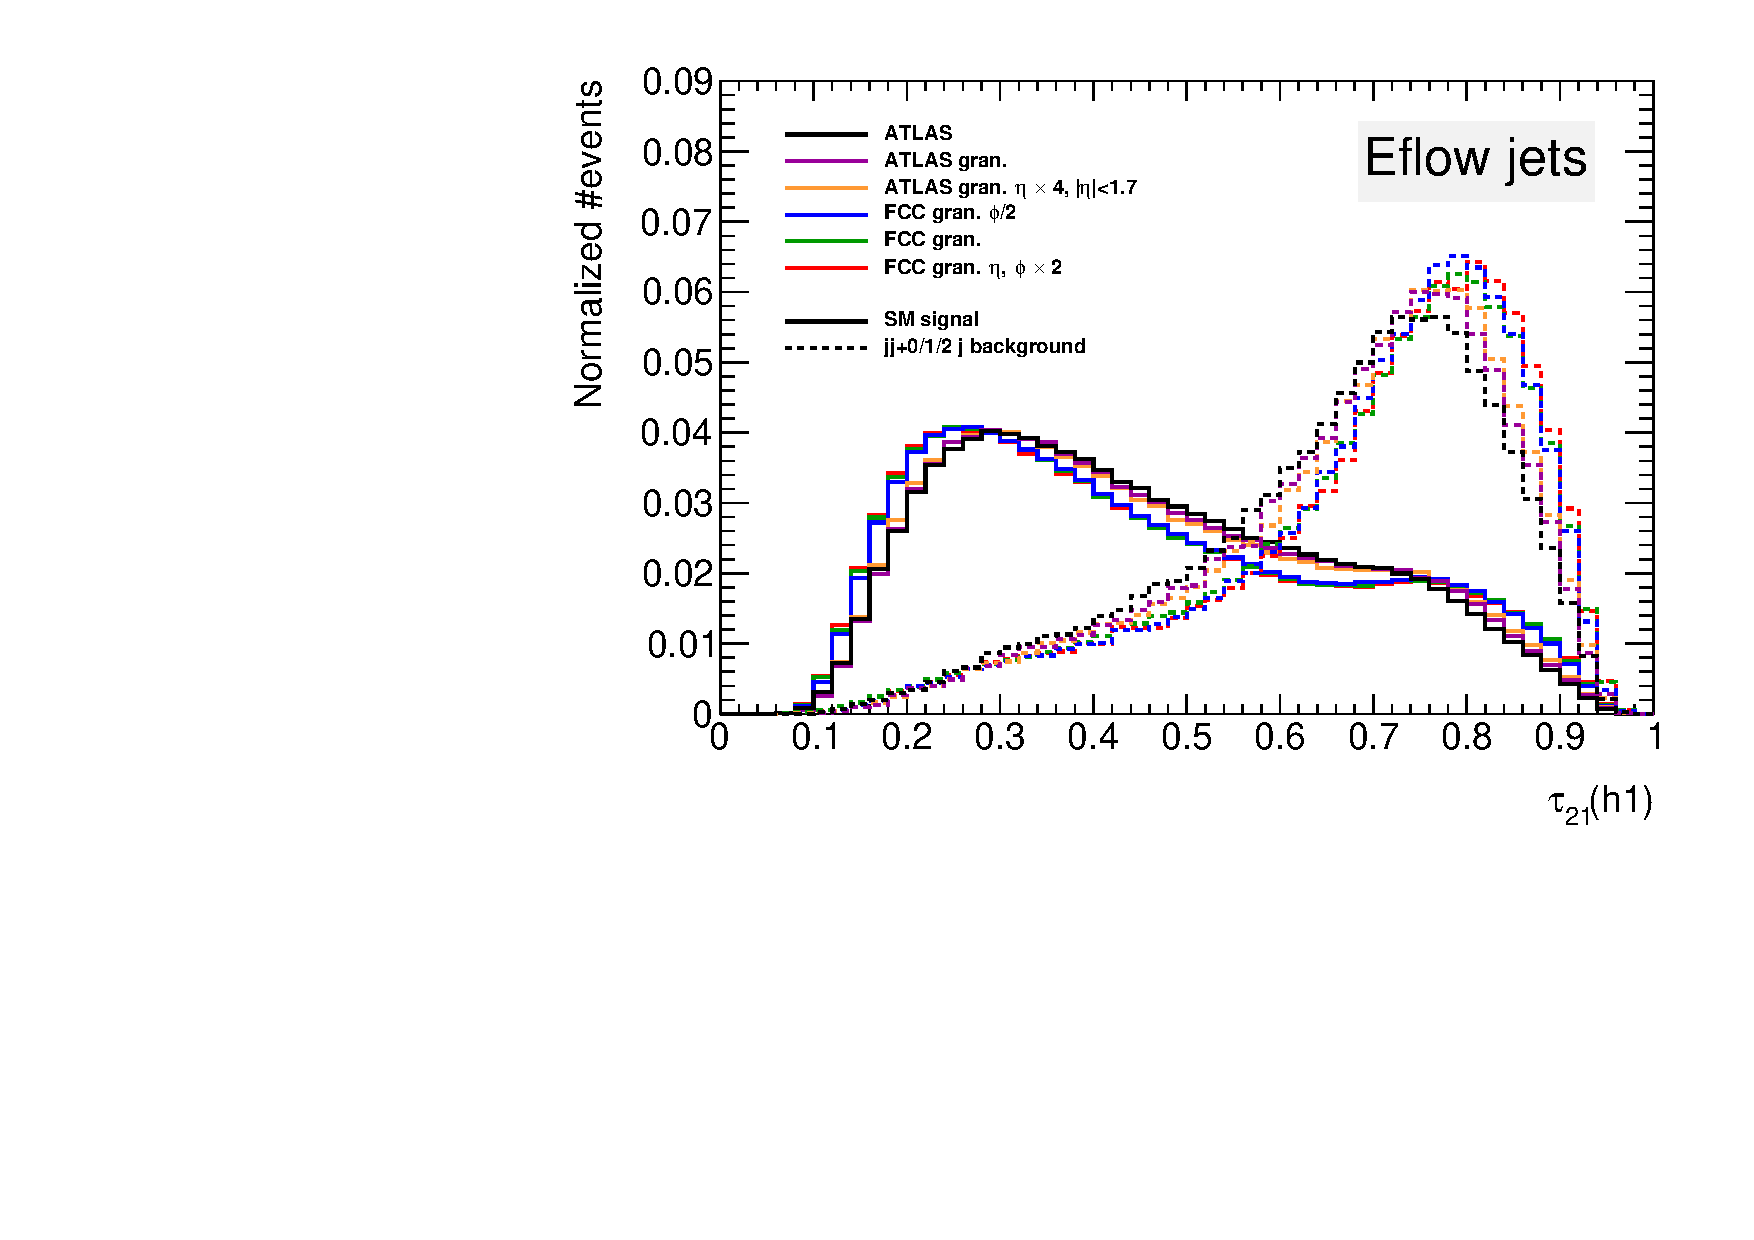
\includegraphics[trim={.65cm 0 0 0},clip,width=\linewidth]{./Figures/tau21_jj.pdf}
		%\caption{oi}
		%\label{fig:h1_pt}
	\end{minipage}%
	\begin{minipage}{.5\textwidth}
		\centering
		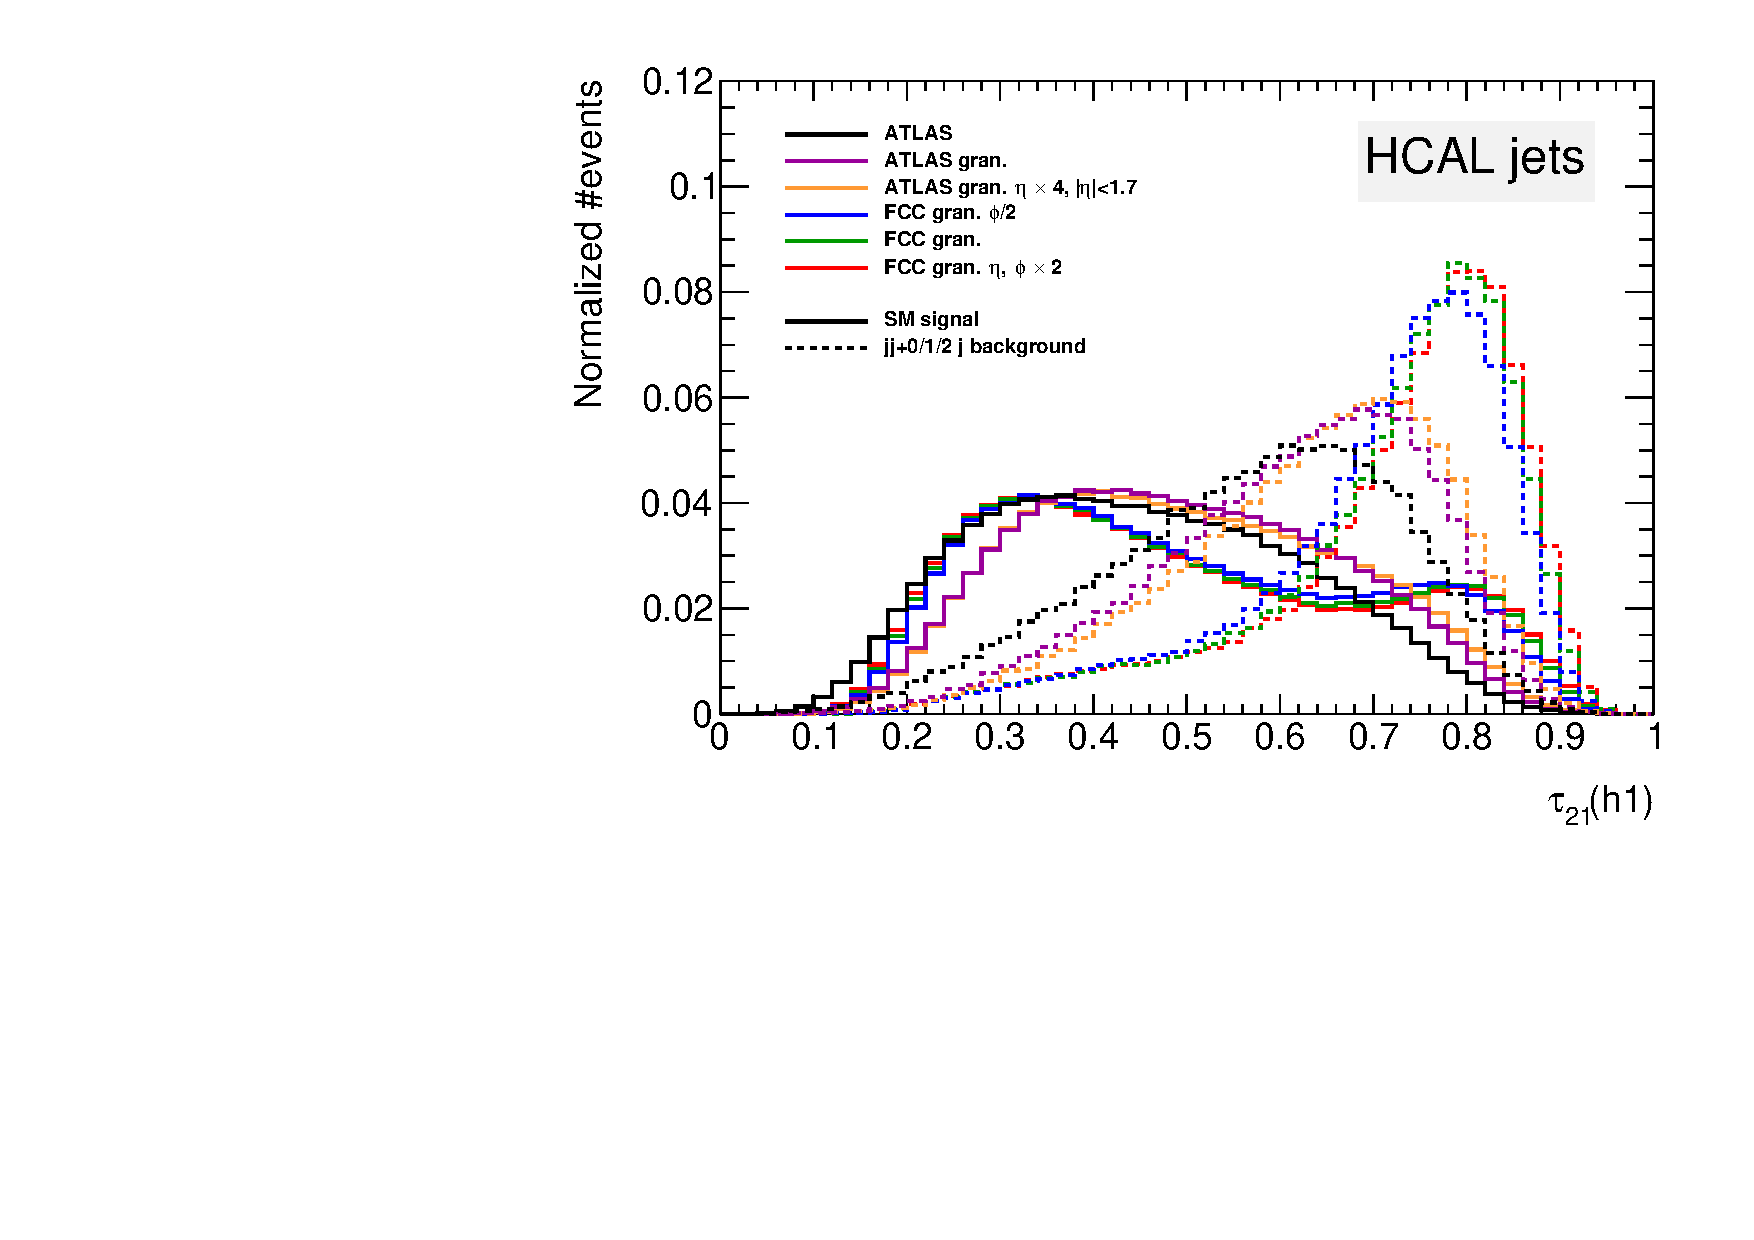
\includegraphics[trim={0 0 .65cm 0},clip,width=\linewidth]{./Figures/tau21CALO_jj.pdf}
		%\caption{oi}
		%\label{fig:h2_pt}
	\end{minipage}
	\begin{minipage}[t]{0.5\textwidth}
		\caption*{(a)}
		%\label{fig1}
	\end{minipage}%%%
	\hfill
	\begin{minipage}[t]{0.5\textwidth}
		\caption*{(b)}
		%\label{fig2}
	\end{minipage}
	\caption{(a) Leading Higgs candidate $\tau_{21}$ distribution for eflow jets and for HCAL jets (b). The colors indicate the different detector configurations. The distributions are shown for the signal (filled lines) and for the $jj+0/1/2~j$ background (dashed lines).}
	\label{fig:tau_sep_jj}
\end{figure} 

\begin{figure}[h]
	\centering
	\begin{minipage}{.5\textwidth}
		\centering
		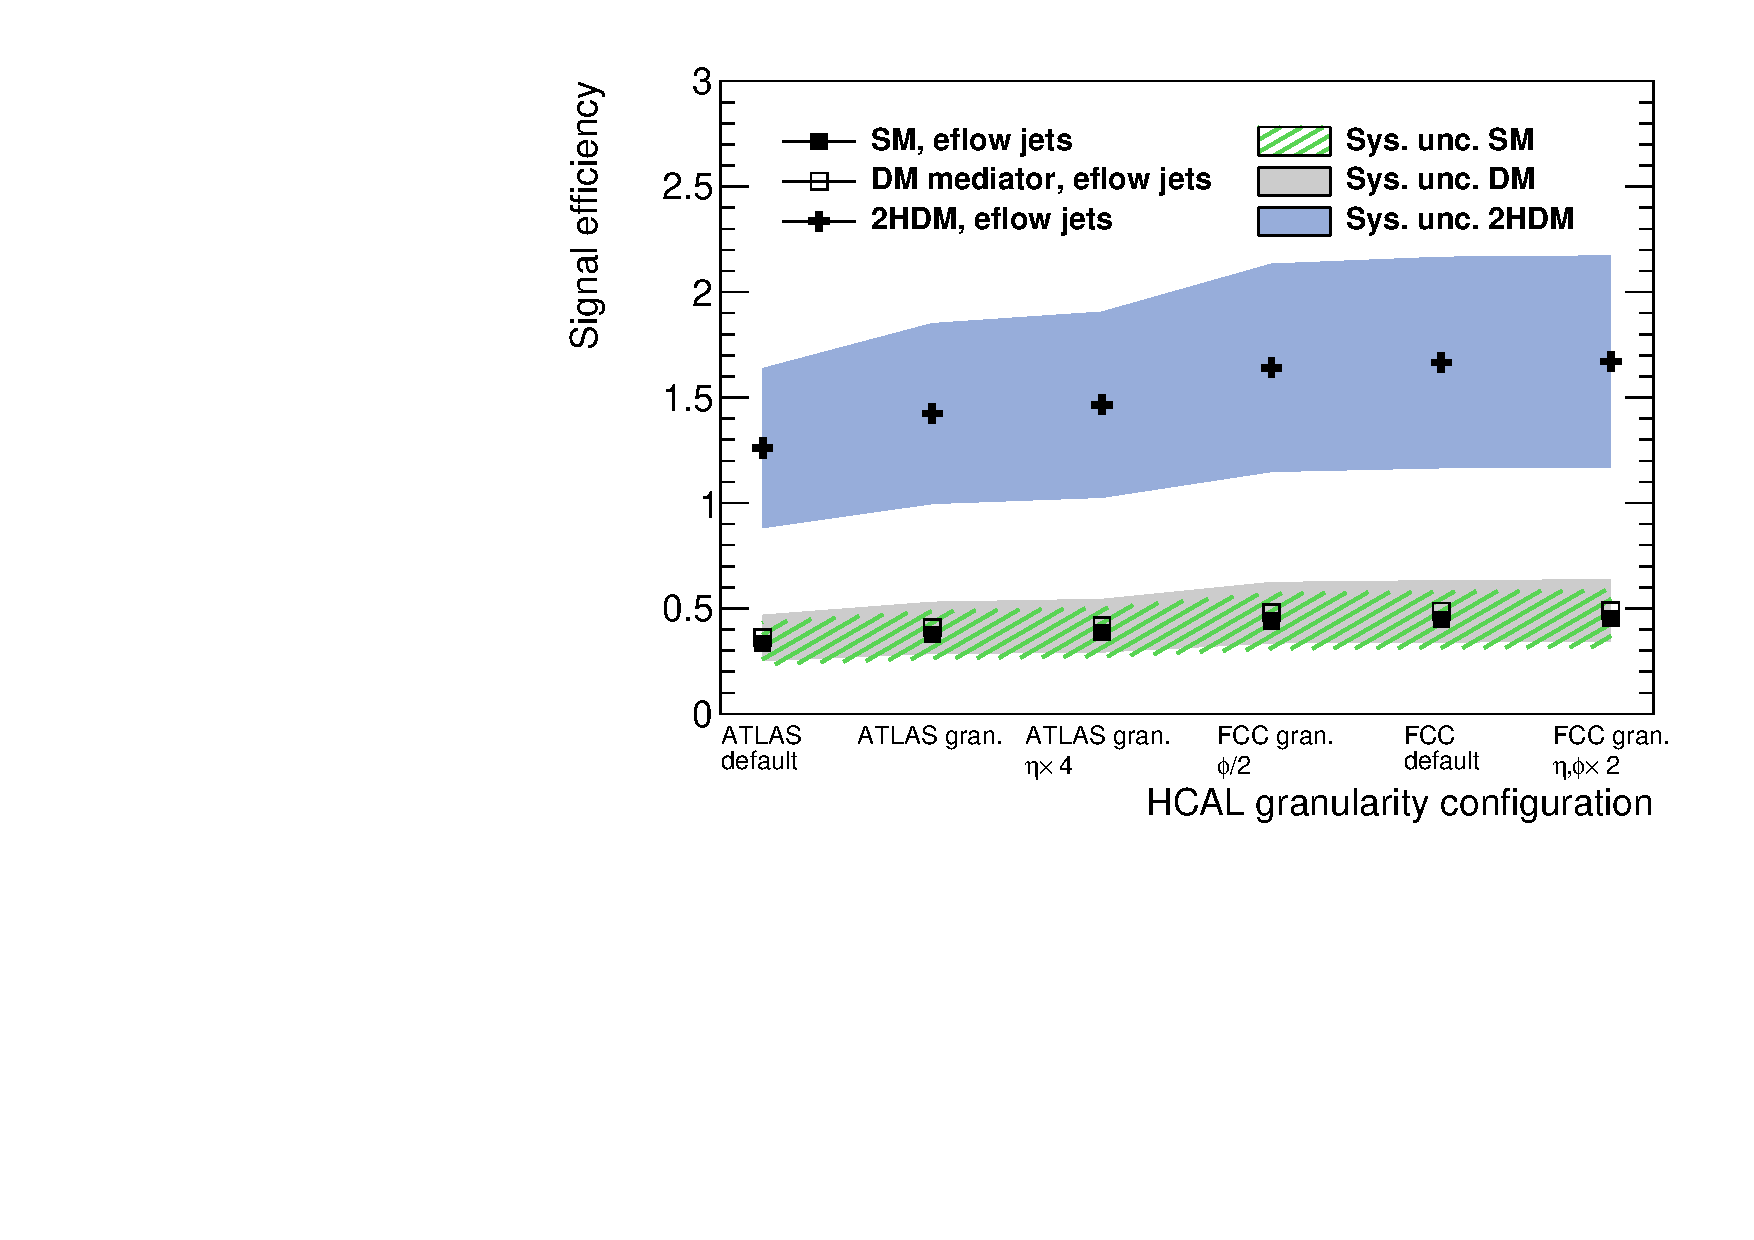
\includegraphics[trim={.65cm 0 0 0},clip,width=\linewidth]{./Figures/EffvsGran_PFjets_Opt.pdf}
		%\caption{oi}
		%\label{fig:h1_pt}
	\end{minipage}%
	\begin{minipage}{.5\textwidth}
		\centering
		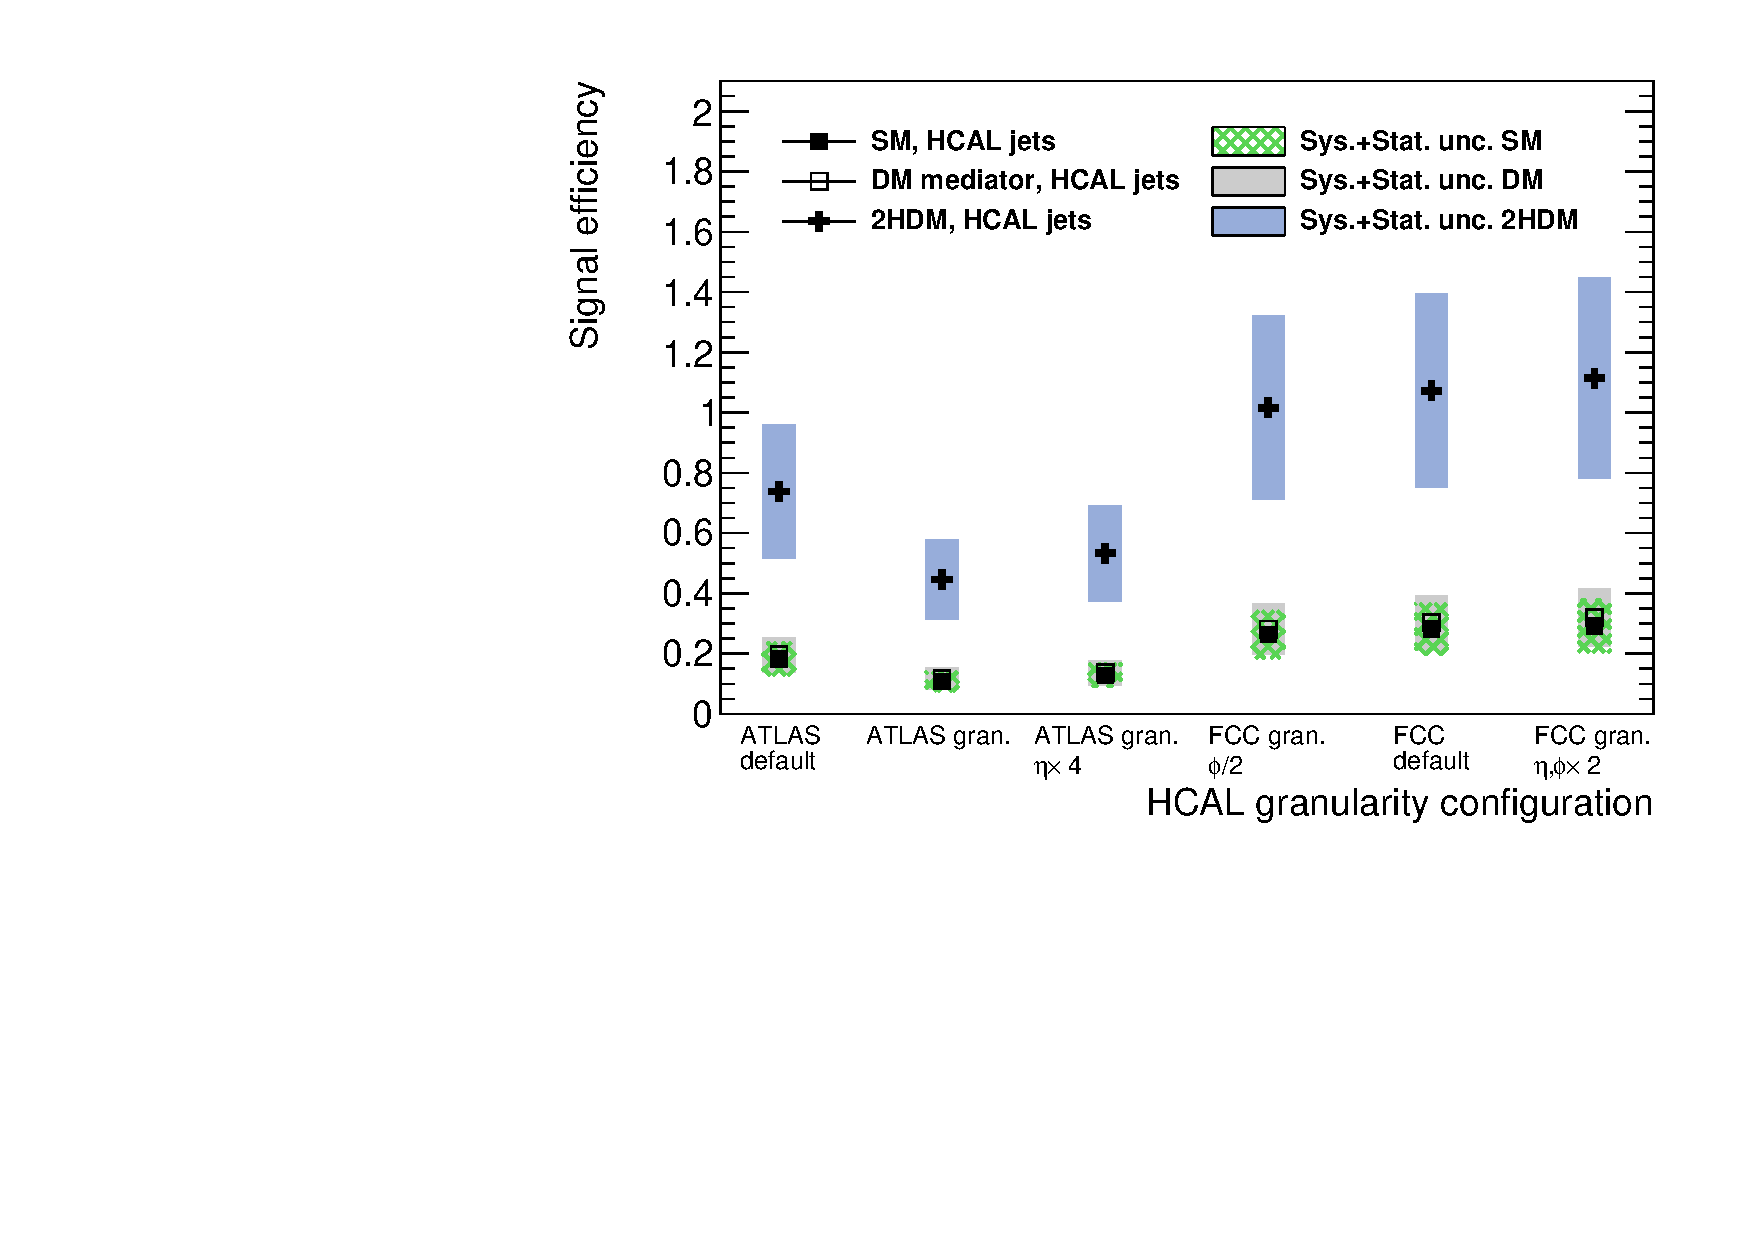
\includegraphics[trim={0 0 .65cm 0},clip,width=\linewidth]{./Figures/EffvsGran_CALOjets_Opt.pdf}
		%\caption{oi}
		%\label{fig:h2_pt}
	\end{minipage}
	\begin{minipage}[t]{0.5\textwidth}
		\caption*{(a)}
		%\label{fig1}
	\end{minipage}%%%
	\hfill
	\begin{minipage}[t]{0.5\textwidth}
		\caption*{(b)}
		%\label{fig2}
	\end{minipage}
	\caption{Signal efficiency as a function of the detector configuration for particle flow jets (a) and for calorimeter jets (b). Three signal models are shown: SM (filled squares), $1$ TeV DM mediator (empty squares) and type II 2HDM with $m_H=900$ GeV (crosses). The error bars are drawn but are smaller than the markers.}
	\label{fig:eff}
\end{figure} 
	



